\section{Exploring Inward-Directed Photon Emission Using Radio Polarization Data of PSR J1705$-$1906}
\paperref{This section is based on work done for private corresponds in relation to
``Six Faint $\gamma$-Ray Pulsars Seen with the {\it Fermi} Large Area Telescope. 
Towards a Sample Blending into the Background'' 
\citep{hou2014six}.}

In the previous section, we discussed extensively the application
of a bidirectional model to the data of PSR J1057$-$5226.
We additionally applied the bidirectional model to the
polarization position angle data of PSR J1705$-$1906
and will discuss the results in this section along with
giving an overview of past studies of this pulsar.
Overall, the results of the analysis of 
PSR J1705$-$1906 are not as compelling or 
conclusive as those of PSR J1057$-$5226 but
are nevertheless reported here for completion.

\subsection{Past Studies}
The pulsar PSR J1705$-$1906 (PSR B1702$-$19) has been identified by \cite{weltevrede2007main}
as a possible candidate for bidirectional emission.
The second component of the main pulse (as labeled by \cite{weltevrede2007main} 
and the pulse with the highest intensity) and the interpulse 
have a phase locked delay.  The main pulse modulation lags that of the
interpulse by $0.43$ rotation period, around the $0.5$ rotation period expected from a geometric delay.
These modulations occur approximately every $10.4$ rotation periods.

\cite{weltevrede2007main} explored evidence of two-pole emission in the
polarization data.  As  \cite{weltevrede2007main} 
noted, a U-shape in the interpulse polarization
data is difficult to model and they fit the polarization
data to the rotating vector model (RVM) both including and excluding
this difficult section.
They further restrict their fits using beaming radius and
width of emission phase arguments.  They also
discuss a single wide cone model.  For the RVM, 
emission from a single wide cone, from both poles, and from a single
pole with bidirectional photons will
have the same polarization sweep due to the lack of relativistic and sweep-back effects.
In order to create a single wide cone model they restrict
$\phi$ (the location in phase of model phase zero) to 
vary between $125^\circ$ and $215^\circ$.  
Fits with these constraints yield $\chi^2$ far worse
than those of a two pole model.

Further, \cite{weltevrede2007main}
examined the inner and outer cone model of \cite{gil1985interpulse}.
With radius beam arguments, they estimate
the difference in emission height between the two
emission regions for this model to be $900$ km
($0.064R_{\rm{LC}}$) which should correspond to a difference in 
phase of $7^\circ$ (see Section \ref{sec:beamingGeometry}
for beaming model details).  Any difference in phase between the 
interpulse and main pulse is much smaller and they therefore
ruled out this model.

Finally for bidirectional  
emission, we would again expect a delay in phase
for any configuration other than the simplest configuration.
This is not seen in the data.  The difference between
the centroid of the interpulse and the minimum between 
the two main pulse components is nearly $180^\circ$.
Alternatively, the phase difference between the two {\it modulating}
components is $176^{\circ}$.  Again using radius beam arguments
and time delay arguments, \cite{weltevrede2007main} gave 
emission height estimates.


\subsection{Polarization Analysis}

\begin{figure}[t!!]
\begin{center}
\includegraphics[width=0.98\textwidth]{chapters/inwardDirectedPhotons/figures/mapB1702allForward.eps}
\caption[The $\chi^2$ map in the $\alpha$-$\zeta$ plane
for fitting polarization sweep data from PSR J1705$-$1906
to a model with only outward-directed photon emission
from two poles]{
The $\chi^2$ map in the $\alpha$-$\zeta$ plane 
for fitting polarization sweep data from PSR J1705$-$1906
to a model with only outward-directed photon emission
from two poles.  
The data fits reasonable well on a wide variety of 
$\alpha$ and $\zeta$ although large $\alpha$ and $\zeta$
are favored.  Red contours are those fits within
$3\sigma$ of the $\chi^2_{\rm{min}}$
with smaller altitudes of emission and
cyan contours are those fits within
$3\sigma$ of the $\chi^2_{\rm{min}}$ with larger 
altitudes of emission.
Black contours are those fits within
$3\sigma$ of the $\chi^2_{\rm{min}}$
and assume only the classical 
open field line emission.
Green contours, on the other hand, allow for
$\rho_{\rm{ypt}}$ as low as $0.5R_{\rm{LC}}$.
\label{fig:allForward}
}
\end{center}
\end{figure}

\begin{figure}[t!!]
\begin{center}
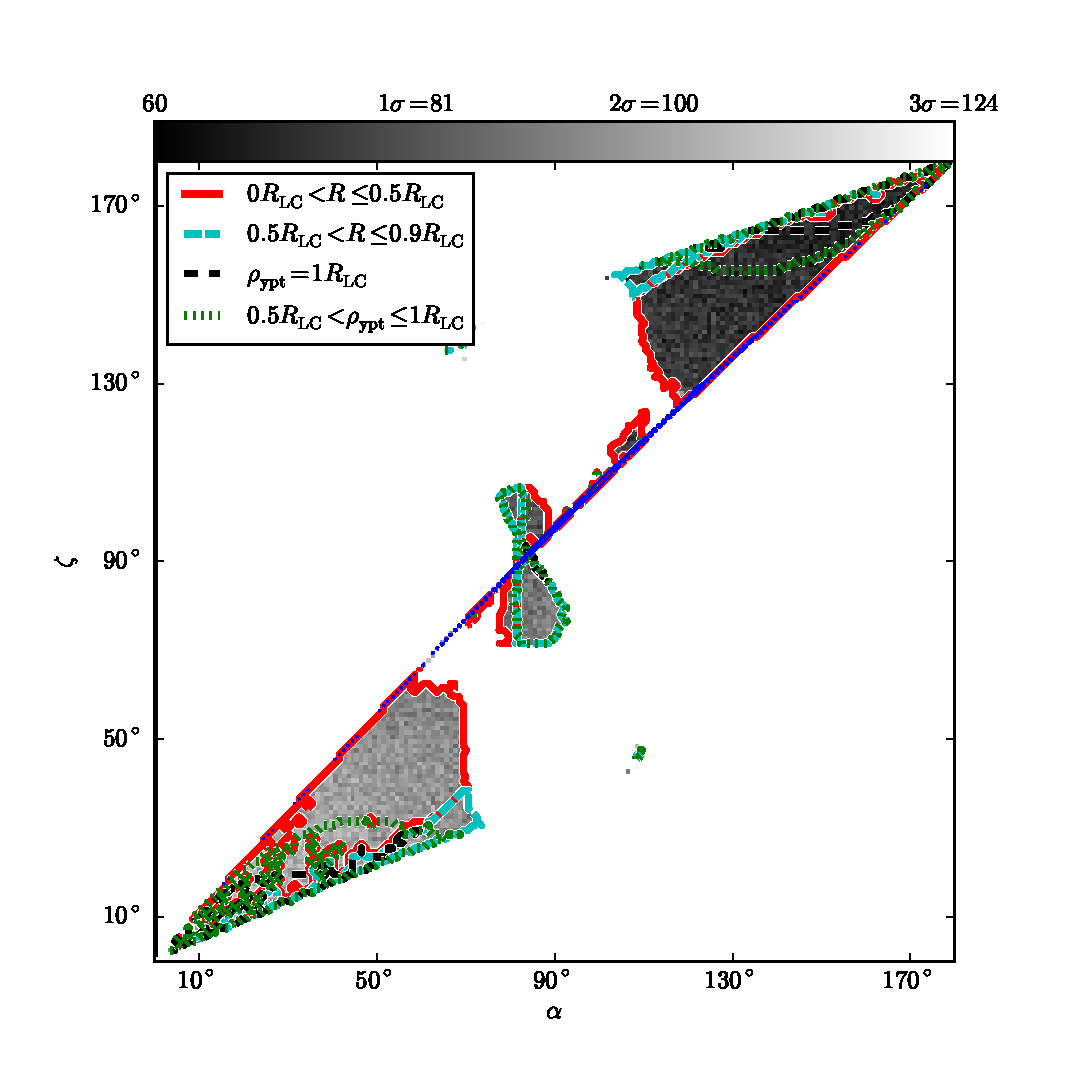
\includegraphics[width=0.98\textwidth]{chapters/inwardDirectedPhotons/figures/mapB1702SinglePole.eps}
\caption[The $\chi^2$ map in the $\alpha$-$\zeta$ plane
for fitting polarization sweep data from PSR J1705$-$1906
to a model with only outward-directed photon emission
from a single pole]{
The $\chi^2$ map in the $\alpha$-$\zeta$ plane
for fitting polarization sweep data from PSR J1705$-$1906
to a model with only outward-directed photon emission
from a single pole.
The data fits reasonable well on a wide variety of
$\alpha$ and $\zeta$ although large $\alpha$ and $\zeta$
are favored.  The region is also more
constrained compared to the two-pole fit.
Red contours are those fits within
$3\sigma$ of the $\chi^2_{\rm{min}}$
with smaller altitudes of emission and
cyan contours are those fits within
$3\sigma$ of the $\chi^2_{\rm{min}}$ with larger
altitudes of emission.
Black contours are those fits within
$3\sigma$ of the $\chi^2_{\rm{min}}$
and assume only the classical
open field line emission.
Green contours, on the other hand, allow for
$\rho_{\rm{ypt}}$ as low as $0.5R_{\rm{LC}}$.
\label{fig:singlePole}
}
\end{center}
\end{figure}

\begin{figure}[t!!]
\begin{center}
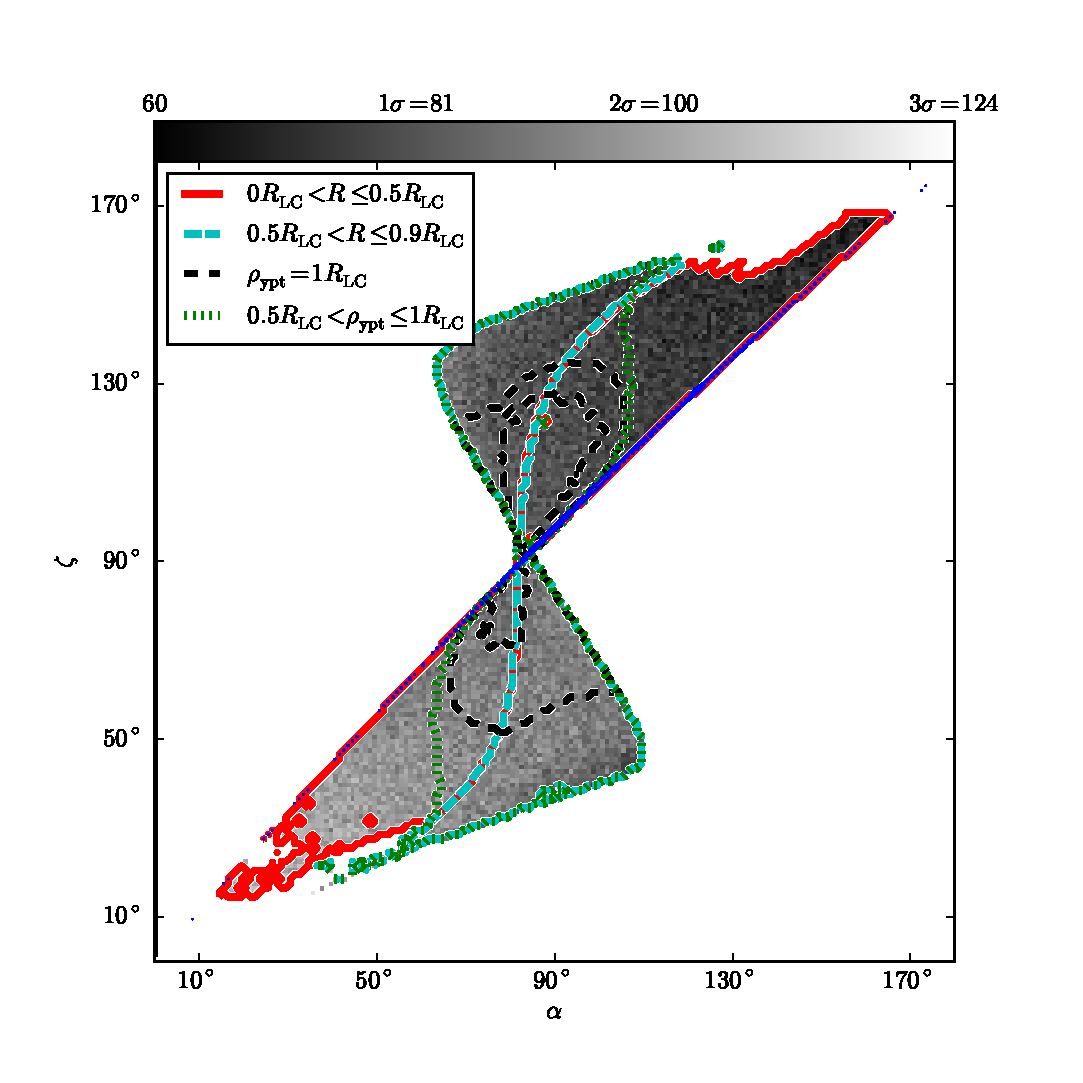
\includegraphics[width=0.98\textwidth]{chapters/inwardDirectedPhotons/figures/mapB1702IPBackward.eps}
\caption[The $\chi^2$ map in the $\alpha$-$\zeta$ plane
for fitting polarization sweep data from PSR J1705$-$1906
to a model with bidirectional photons from a single pole]{
The $\chi^2$ map in the $\alpha$-$\zeta$ plane
for fitting polarization sweep data from PSR J1705$-$1906
to a model with bidirectional photons from a single pole.
Again, the data fits reasonable well on a wide variety of
$\alpha$ and $\zeta$. Large $\alpha$ and $\zeta$
are favored although not as large as those for the 
previous two fitting schemes (all outward-directed emission
and single pole emission).  Red contours are those fits within
$3\sigma$ of the $\chi^2_{\rm{min}}$
with smaller altitudes of emission and
cyan contours are those fits within
$3\sigma$ of the $\chi^2_{\rm{min}}$ with larger
altitudes of emission.
Black contours are those fits within
$3\sigma$ of the $\chi^2_{\rm{min}}$
and assume only the classical
open field line emission.
Green contours, on the other hand, allow for
$\rho_{\rm{ypt}}$ as low as $0.5R_{\rm{LC}}$.
\label{fig:inward}
}
\end{center}
\end{figure}

Here we present our own analysis of the 1.408 GHz polarization 
data \citep{gould1998multifrequency} using the multiple-altitude model
with bidirectional photon emission.
Similar to \cite{weltevrede2007main}, three scenarios are
examined: emission from two poles emitting only forward-directed
photons, emission from a single wide pole emitting only forward-directed
photons, and emission from a single pole with bidirectional photons (both inward-
and outward-directed).  For the latter case, the peak identified as the interpulse
is assumed to originate from inward-directed photons.

Figure~\ref{fig:allForward}
shows fit results for pulsar PSR J1705$-$1906 
for the typical configuration with emission from
two separate poles for the two different pulses.
Figure~\ref{fig:singlePole}
shows fit results for a configuration where
emission originates from a single wide pole.
Figure~\ref{fig:inward}
shows fit results for a configuration where 
polarization of the ``main pulse'' as identified by \cite{weltevrede2007main}
originates from outward-directed photons and 
``interpulse'' polarization originates from the same pole 
but from inward-directed photons.
Also shown on the graphs are contours for high and low altitude cuts,
classical open zone constraints ($\rho_{\rm{ypt}}=1R_{\rm{LC}}$),
and restricted y-point lowering constraints in which emission is allowed from
the closed zone.
Overall, the results are not very constraining.
All three fits have $\chi^2_{\rm{min}}\sim60$ for DOF$=22-5$.
Also note that only a single altitude was applied for all components of the
polarization sweep.  Allowing for multiple altitudes would make the
fitting even less constraining.
The long, thin contour along the diagonal of the graphs 
is the RVM fit.  For the RVM fitting, $\chi^2_{\rm{min}}=65$ such
that the use of finite altitudes is not well justified statistically.

Although $\gamma$-ray fitting is not formally performed,
\cite{hou2014six} notes using results from \cite{Watters:2010jb}
some constraints to the fit parameters.
They conclude that $\alpha>50^\circ$ and $\zeta<60^\circ$
although this too is not very constraining.  Overall,
better data is likely needed to make more meaningful
conclusions about PSR J1705$-$1906 and the possibility of
inward-directed photon emission.

